% Options for packages loaded elsewhere
\PassOptionsToPackage{unicode}{hyperref}
\PassOptionsToPackage{hyphens}{url}
%
\documentclass[
]{article}
\usepackage{lmodern}
\usepackage{amssymb,amsmath}
\usepackage{ifxetex,ifluatex}
\ifnum 0\ifxetex 1\fi\ifluatex 1\fi=0 % if pdftex
  \usepackage[T1]{fontenc}
  \usepackage[utf8]{inputenc}
  \usepackage{textcomp} % provide euro and other symbols
\else % if luatex or xetex
  \usepackage{unicode-math}
  \defaultfontfeatures{Scale=MatchLowercase}
  \defaultfontfeatures[\rmfamily]{Ligatures=TeX,Scale=1}
\fi
% Use upquote if available, for straight quotes in verbatim environments
\IfFileExists{upquote.sty}{\usepackage{upquote}}{}
\IfFileExists{microtype.sty}{% use microtype if available
  \usepackage[]{microtype}
  \UseMicrotypeSet[protrusion]{basicmath} % disable protrusion for tt fonts
}{}
\makeatletter
\@ifundefined{KOMAClassName}{% if non-KOMA class
  \IfFileExists{parskip.sty}{%
    \usepackage{parskip}
  }{% else
    \setlength{\parindent}{0pt}
    \setlength{\parskip}{6pt plus 2pt minus 1pt}}
}{% if KOMA class
  \KOMAoptions{parskip=half}}
\makeatother
\usepackage{xcolor}
\IfFileExists{xurl.sty}{\usepackage{xurl}}{} % add URL line breaks if available
\IfFileExists{bookmark.sty}{\usepackage{bookmark}}{\usepackage{hyperref}}
\hypersetup{
  hidelinks,
  pdfcreator={LaTeX via pandoc}}
\urlstyle{same} % disable monospaced font for URLs
\usepackage[margin=1in]{geometry}
\usepackage{graphicx}
\makeatletter
\def\maxwidth{\ifdim\Gin@nat@width>\linewidth\linewidth\else\Gin@nat@width\fi}
\def\maxheight{\ifdim\Gin@nat@height>\textheight\textheight\else\Gin@nat@height\fi}
\makeatother
% Scale images if necessary, so that they will not overflow the page
% margins by default, and it is still possible to overwrite the defaults
% using explicit options in \includegraphics[width, height, ...]{}
\setkeys{Gin}{width=\maxwidth,height=\maxheight,keepaspectratio}
% Set default figure placement to htbp
\makeatletter
\def\fps@figure{htbp}
\makeatother
\setlength{\emergencystretch}{3em} % prevent overfull lines
\providecommand{\tightlist}{%
  \setlength{\itemsep}{0pt}\setlength{\parskip}{0pt}}
\setcounter{secnumdepth}{-\maxdimen} % remove section numbering

\author{}
\date{\vspace{-2.5em}}

\begin{document}

\hypertarget{methodology}{%
\section{Methodology}\label{methodology}}

The concept of missing data is ubiquitous within academic disciplines
and often complicates innumerable types of real-world studies. Missing
data will be defined within this thesis as \emph{occurences within a
dataset where there is no value stored for a variable in the observation
of interest}. As most studies often utilize data collected through
mediums such as surveys, questionnaires, or field research, missing data
is an unavoidable problem. Missing data hinders one's ability to work
with and analyze the phenomena at hand, as data is often the basis of
all studies. One of the most glaring issues with missingness is how it
can introduce bias within an analysis, which can more often than not,
invalidate a study if not accounted for and handled properly.
Missingness can often be detrimental to data quality which can result in
increased uncertainty with any types of performed analysis
{[}@Hall2020{]}.

This thesis will go into a more specific instance of missing data known
as censoring, which is \emph{the condition when one has only partial
information regarding the values of a measurement within a dataset}. We
will introduce and define the three types of censored data, challenges
with the reporting of censored data, alongside a discussion on common
statistical approaches to handling censored data.

\hypertarget{censored_data}{%
\subsection{Censored Data}\label{censored_data}}

As discussed previously, censored data is a specific type of missingness
where one has only partial information regarding the values of a
measurement in a dataset. There are many types of censoring which can
occur, but three main ones which are the most common: right censoring,
interval censoring, and left censoring.

\hypertarget{right}{%
\subsubsection{Right Censoring}\label{right}}

Right censoring is a specific instance in which we only know that the
true value of a data point lies above a certain threshold, but it is
unknown by how much. Suppose a study on income and mortality is
conducted with the variable of interest, \(T\), being the time measured
from the start of the study to the death of the participant. The study
has a duration of 5 years, in which participants are expected to submit
a form regarding their annual income. The value for the participant
would be considered to be right-censored if at any point during the
study, they failed to follow-up, or if the participant was still alive
at the conclusion of the 5 year study. In this design study, several
possibilities can occur, illustrated in Figure
@ref(fig:rightcensoringexample).

\begin{figure}
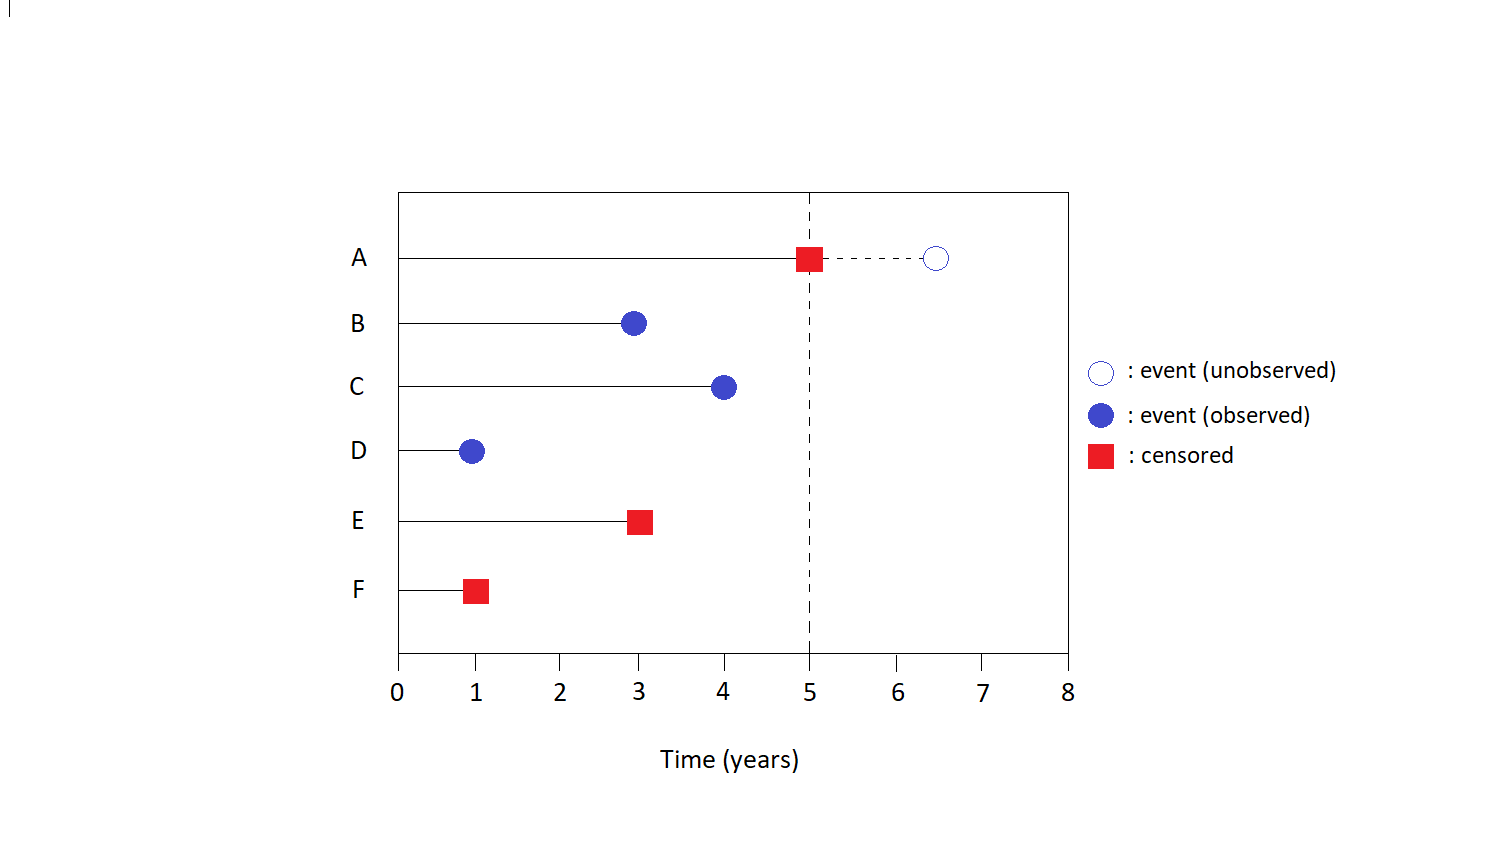
\includegraphics[width=1\linewidth]{figures/right_censoring_example} \caption{Right Censoring Example}\label{fig:rightcensoringexample}
\end{figure}

As illustrated by individual A in Figure
@ref(fig:rightcensoringexample), this individual lives on until the
termination of the study. We don't know at what point they passed away
exactly, since they didn't pass away during the time constraints of the
study. As such, the only information we have is \(T > 5\).

If an individual does pass away at some point, \(t_i\), \emph{during}
the study, then \(T = t_i\). This can be illustrated within Figure
@ref(fig:rightcensoringexample) by individuals B, C, and D for which
\(T = 3\), \(T = 4\), and \(T = 1\).

There is a final possibility for individuals who choose to censor
themselves. Illustrated in Figure @ref(fig:rightcensoringexample) by
individuals E and F, we can see that they are marked as censored at
\(T = 3\) and \(T = 1\), respectively. These individuals may have chosen
to stop submitting information to the study or drop out of the study
entirely without warning. As we have no information about whether or not
if they died or simply did not submit their form, all we know is that
the individual died/will die at some point after the point at which they
were censored.

Right censoring is the most common type of censoring and can often be
found in clinical trial studies, mortality studies, and other forms of
surival analyses.

\hypertarget{left}{%
\subsubsection{Left Censoring}\label{left}}

\begin{figure}
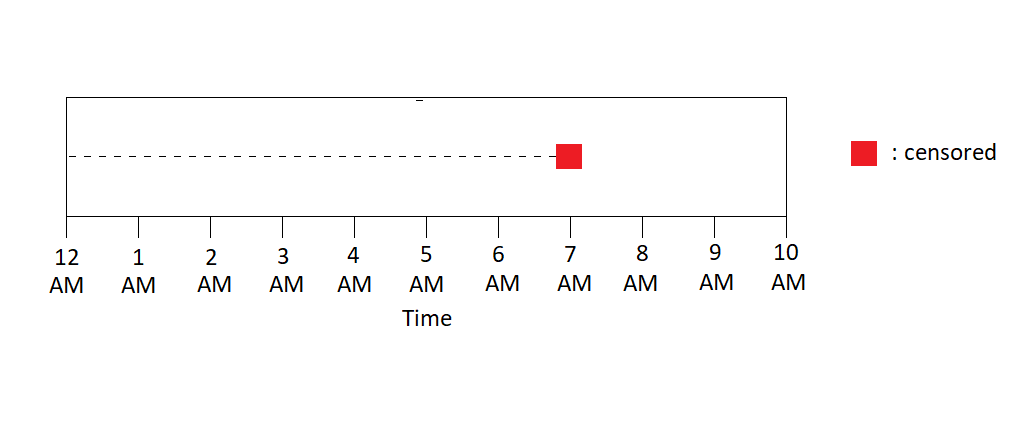
\includegraphics[width=1\linewidth]{figures/left_censoring_example_fix} \caption{Left Censoring Example}\label{fig:leftcensoringexample}
\end{figure}

In contrast with right censoring, left censoring is a specific instance
of censoring in which we only know that the true value of a data point
falls below a certain threshold which we call the \emph{limit of
detection} (LOD).

To understand this concept better, consider the following example.
Imagine a scenario in which you are attempting to estimate the time at
which the sun rises each morning. You plan to wake up every morning far
before the sun rises, but on the first day of the study, you oversleep
and wake up at 7:00 A.M. with the sun already out. We now have an
instance of left-censored data. We want to know the time at which the
sun rose, but all we have is an upper limit (7:00 A.M.).

Left censoring is commonly found in environmental, water quality, and
chemical-related research where the focus is on the concentration of an
analyte. Due to limitations on measuring instruments, left censored data
are commonly found in these types of studies. The most pressing issue of
left-censored data mostly lie in the difficulty of distinguishing
between extremely low values and statistical noise {[}@Hall2020{]}.

\hypertarget{interval}{%
\subsubsection{Interval Censoring}\label{interval}}

\begin{figure}
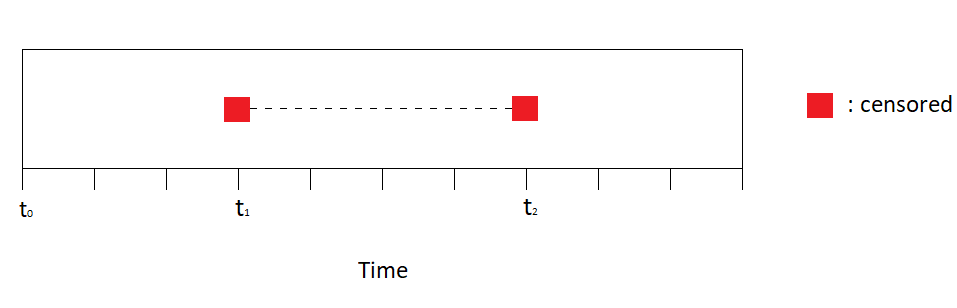
\includegraphics[width=1\linewidth]{figures/interval_censoring_example_fix} \caption{Interval Censoring Example}\label{fig:intervalcensoringexample}
\end{figure}

Interval censoring is another form of censoring in which the random
variable of interest is known to be between an interval of two values.
Considering a random variable \(T\), which denotes the survival time of
interest, if interval censoring is at hand, we can denote the interval
containing \(T\) to be \(I = [t_1, t_2]\), with \(t_1\) being the
beginning of the interval and \(t_2\) being the end of the interval.

Left and right censoring are special cases of interval censoring. In the
case of left censoring, \(t_1 = 0\); and conversely in the case of right
censoring, \(t_2 = \infty\).

To conceptualize interval censoring, we can consider a example study on
virus testing in which participants get their blood drawn in order to
detect whether or not they test positive for a virus or not. The random
variable in question is \(T\), which represents the exact timepoint at
which the subject contracted the virus. If an individual was first
tested at time \(t_1\) and tested negative, but was tested again at a
later time \(t_2\) and tested positive, the specific time \(t\) at which
the subject contracted the virus is unknown. All we know is that it lies
somewhere between the interval, \(I = [t_1, t_2]\), but not the exact
time at which they contracted it.

There are a myriad of types of censoring which can be discussed, however
the focus of my thesis deals specifically with the challenges of
reporting these values alongside methods of handling left-censored data.

\hypertarget{challenges}{%
\subsection{Challenges of Reporting Censored Data}\label{challenges}}

There is no universal reporting practice for values below the LOD which
can lead to confusion amongst researchers. The lack of standardization
makes it difficult to distinguish LOD values with uncensored values.
This can lead to LOD values unintentionally being overlooked, causing
faulty analysis or conclusions which are heavily flawed.

In a study involving the precision of lead measurements near
concentrations of the limit of detection, Berthouex (1993) discusses the
disparity in practices within chemists on ways to record LOD values. He
enumerates in a following list, common reporting practices in this
field:

\begin{enumerate}
  \item Reporting the trace, a chemical whose average concentration is less than 100 $\mu g$
  \item Reporting  the letters ND, which stand for "not detected"
  \item Reporting the numerical LOD value itself
  \item Reporting "<", followed by the numerical LOD value
  \item Reporting some value between 0 and the LOD value, such as one-half the LOD value
  \item Reporting the actual measured concentration, even if it falls below the LOD
  \item Reporting the actual measured concentration, followed by "(LOD)"
  \item Reporting the actual measured concentration with a precision ($\pm$) statement
\end{enumerate}

The latter three methods are the best procedures to follow, especially
from a practical and statistical point of view according to Gilbert
(1987). He argues that assuming the small concentration values are not
from some sort of measurement error during data collection, then the
value holds value. As such, recording a measurement as ``below LOD,''
without any sort of accompanying value would be discarding useful
information which could have been used in practice and analysis.

Berthouex (1993) discusses the prevalence in regards to the practice of
censoring data by reporting only values which are above the detection
limit and discarding those which fail to yield quantifiable results. He
discourages this practice and instead suggests the reporting of
measurements, even when those values are below the limit of detection.

Further supporting the stance of keeping all concentration values rather
than only those above the detection limit, Monte-Carlo experiements
conducted by Gillom (1984) show that linear trends in water-quality data
were far more easily able to be detected with uncensored data as
compared to censored data. The methods they used to handle censored
water quality data were found to produce wild and erratic estimates for
the mean and standard deviation of datasets with higher censoring levels
than those without. They found a general trend of decreasing
classification success with increased censoring levels, attributing it
to the limited availability of information in censored data.

\hypertarget{Approaches}{%
\subsection{Approaches}\label{Approaches}}

It is important to note that the values below the LOD still contain
information, specifically that the values is between the lower bound
value (if it exists) and the LOD {[}@Chen2011{]}. As such, there are a
variety of statistical treatments to handle censored data which have
been popularized in the statistical literature which will be discussed
within this section.

Omission involves the deletion of data points which are deemed to be
invalid as a result of left-censoring or any other deficiencies in the
data. This is also more commonly known as \emph{available-case
analysis}, in which statistical analysis is conducted while only
considering the observations which have no missing data on the variables
of interest, and excluding the observations with missing values
{[}@May2012{]}. May argues against this approach and claims that the
loss of information from discarding data and the inflation of standard
errors of estimates (when discussing missingness in a regression
context) will invariably be inflated as a result of the decreased sample
size. The advantages of omission lies in its ease of implementation.

Apart from available-case analysis, over the past century, a myriad of
methods to deal with censoring have been developed to counter this issue
-- some more statistically sound than others. We will review some of the
most common methods to estimate descriptive statistics involving
censored data, which include: substitution, maximum likelihood
estimation, Kaplan-Meier, and regression on order statistics
{[}@Lafleur2011{]}.

\hypertarget{Substitution}{%
\subsubsection{Substitution Method}\label{Substitution}}

Often condemned in papers as a statistically unsound method to handle
censored data, substitution methods are ubiquitous in the chemical and
environmental sciences as an appropriate and recommended method to work
with left-censored chemical concentration data {[}@Canales2018{]}.

The substitution method simply involves imputing in a replacement value
in lieu of the censored data point. The lack of a global, standardized
replacement value to substitute is one of the most pronounced downside
of this method. The replacement value used may differ between studies
but common values include: \(\frac{LOD}{2}, \frac{LOD}{\sqrt2}\), or
\(LOD\) {[}@Lee2005{]}. Different disciplines have their own suggested
``best'' replacement value to use, an example being \(\frac{3}{4}\)
times the LOD being a common replacement value in geochemistry
{[}@Crovelli1993{]}. However, it must be recognized that the
substitution method is a statistically unsound technique which is often
used in non-rigorous statistical settings due to them being quite easy
to implement {[}@Chen2011{]}. As such, there have been several studies
in order to investigate the effectiveness of the method.

Proponents of the substitution method claim that the replacement value
\(\frac{LOD}{2}\) is useful for data sets in which the majority of the
data are below the LOD or when the distribution of the data is highly
skewed; the definition of ``highly skewed'' being any distribution with
a geometric standard deviation (a measure of spread commonly used in
tandem with log-normal distributions) of 3 or more {[}@Hornung1989{]}.
They also suggest using \(\frac{LOD}{\sqrt2}\) when there are only a few
data points below the LOD or when the data is not highly skewed.

Substitution methods are flawed as they can often introduce a ``signal''
which was not originally present within the data, or even obstruct an
actual signal which was present in the original data {[}@Lee2005{]}.
Numerous authors have advised against the usage of substitution methods
for being statistically inappropriate to use. Glass and Gray (2001)
found that both introduce large errors and biases in descriptive
statistics of interest. Thompson and Nelson (2001) conducted a study in
which they found similar results, in that it often led to biased
parameter estimates and ``artificially small standard error estimates.''
Hewett and Ganser (2007) also found in their simulation study that the
substitution method yielded the lowest average bias and root mean
squared error values (comparison metrics to measure accuracy) in their
estimation of the mean. Overall, the overall consensus seems to advise
against the practice of these substitution techniques.

\hypertarget{MLE}{%
\subsubsection{Maximum Likelihood Estimation Method}\label{MLE}}

Maximum likelihood (ML) estimation is a parametric technique which
allows us to estimate the parameters of a distribution or model when the
data is from a multivariate normal distribution.

To give a brief introduction to the mechanisms of ML estimation, let
\(f(x|\theta)\) denote the probability density function (PDF) which
specifies the probability of observing the random variable \(x\) given
the parameter \(\theta\).

Given a random, independently and identically distributed
(\emph{i.i.d.}) set of random variables \(X_1, X_2,...,X_n\) from
\(f(x|\theta)\), we know that each individual observation \(x_i\)'s are
statistically independent from one another, which allows us to express
the PDF as the product of all individual densities. For every observed
random sample \(x_1,...,x_n\), we can define the joint density function
to be:

\[f(x_1,...,x_n|\theta) = f(x_1|\theta)...f(x_n|\theta) = \prod_{i=1}^{n}f(x_i|\theta)\]
In most real-life scenarios, the actual (observed) data is already
given, and our goal is to find the PDF which is most likely to generate
our observed values. In order to solve this inverse problem, we
introduce the likelihood function, which is defined as the joint density
of the observed data as a function of the parameter (with the data held
as a fixed constant).

In mathematical notation, upon observing the given data,
\(f(x_1,...,x_n|\Theta)\) becomes a function of \(\theta\) alone, so we
obtain a likelihood of:

\[lik(\theta) = f(x_1,...,x_n|\theta)\] It is important to recognize the
difference which separates the likelihood function and the PDF. The PDF
is a function of the observed data given a parameter(s). It gives
information regarding the probability of a particular data value for a
fixed parameter.

On the other hand, the likelihood function is a function of the
parameter, given a set of observed data. It tells us the likelihood of
observing a particular parameter value for a fixed set of data.

Our goal is to obtain the ML estimate of our parameter which maximizes
the likelihood function, \(lik(\theta)\), in other words, to obtain a
\(\theta\) which makes our observed data the most probable.

As we previously declared our random variables \(X_1, X_2,...,X_n\) to
be i.i.d, we can rewrite the likelihood to be a product of the marginal
densities:

\[lik(\theta) = \prod_{i=1}^{n} f(x_i|\theta)\] in which we can then
maximize the likelihood to find the best mle of \(\theta\) to best
capture our observed data.

Yavuz et. al (2017) discuss the usage of MLE method, when missing data
is present, and note that it is only appropriate to use for non-negative
probability distributions such as: exponential, log-normal, normal, and
Weibull.

When left censoring is present, the likelihood function changes in order
to account for both the censored observations and the uncensored
observations and becomes:

\[lik(\theta) = \prod_{i=1}^n f(x_i|\theta)^{\delta_{i}} \ \times F(x_i|\theta)^{1-{\delta_{i}}}\]

in which \(\delta_{i}\) is an indicator, representing whether or not if
the \(i\)th observation is censored or not:

\$\$ \delta\_i =

\begin{cases}
  0, & \text{if censored} \\
  1, & \text{if uncensored}
\end{cases}

\$\$ From this updated definition of the likelihood function which must
be used in the presence of left censored data, it is then possible to
follow typical procedures to find the estimator, \(\theta\), which
maximizes the likelihood, also known as the \emph{maximum likelihood
estimator}. With this knowledge, the evaluation statistics of interest
(mean, variance, etc.) relating to the specified distribution are known.

The MLE method we will be utilizing is actually performed by obtaining
regression estimates of slope(s) and intercepts through maximum
likelihood with censored data. The \texttt{cenmle} function in the
\texttt{NADA} package allows the user to specify censored and uncensored
data, and uses the LOD as the placeholder. As this method is not an
imputation technique, values are not replaced. This method allows us to
calculate the summary statistics for the entire data set -- including
the censored values.

Can also impute values from this distribution (Canales 2018)\ldots{}
{[}expand furhter{]}

As a technique which heavily relies upon knowing a distribution which
best models the data, MLE is one of the most well-known parametric
approaches to handling LOD values. Many studies use the MLE as a sort of
baseline method of handling censored values, to which they compare their
new techniques upon {[}@Ganser2010{]}. However, it must be known that
regardless of the prevalence of the MLE method, it is not free from its
own downfalls. Canales (2018) found that the MLE method seems to
underperform when the data in question was highly skewed, in which
overinflated mean squared errors were often obtained. Being a technique
which is so heavily dependent upon distributional assumptions, an
incorrect specification of the distribution of the censored data will
inevitably lead to misleading results {[}@Bolks2014{]}.

\hypertarget{rkm}{%
\subsubsection{Kaplan-Meier Method}\label{rkm}}

As a phenomenon, censoring is most often discussed in survival analysis,
which concerns itself with techniques to analyze a time to an
\emph{event variable}. As its name suggests, these variables measure the
time which passes until some sort of event occurs. This can be as
innocuous as the time until device breaks, time until birds migrate away
from their homes, time until a person passes away, etc. Regardless of
which, all these scenarios share a common problem in terms of the
possibility of the data being ``censored.''

The Kaplan-Meier (KM) method is a common nonparametric technique used to
deal with censored data. Nonparametric methods do not utilize any
information regarding the parameters for a specified distribution, like
the mean and standard deviation for the normal distribution. The KM
method was originally developed to handle right-censored survival
analysis data. The advantages of the KM method lie in its robustness as
a nonparametric method, it performs well without having to depend upon
distributional assumptions. Many recommend its usage for when there are
cases of severe censoring, instances where \textgreater{} 90\% of the
data is censored {[}@Canales2018{]}.

To introduce the concept of the KM-estimator, it is helpful to take a
look into its usages in survival analysis studies where the focus is
often on a type of ``time to a certain event occurring'', often being
cases such time to death, or time to failure.

The KM-estimator is a nonparametric statistic used to estimate the
survival curve from the empirical data while accounting for the
possibilities of certain values being censored. It does this by assuming
that censoring is independent from the event of interest and that
survival probabilities remain the same in observations found early in
the study and those recruited later in the study.

The KM-estimator when performing an empirical estimation of the survival
curve at time \(t\) can be represented by the following equation:

\[\hat{S}(t) = \prod_{\ t_i \le \ t }\left(1-\frac{d_i}{n_i}\right)\]
where \(t_i\) is the distinct event time, \(d_i\) is the number of event
occurrences at time \(t_i\), and \(n_i\) is the number of followup times
(\(t_i\)) that are \(\ge\) \(t_i\) (how many observations in sample
survived at least/or past the time \(t_i\)) {[}@Klein2003{]}.

Typically, the KM-estimator can only be used to estimate the
distribution function of right-censored data, in which a data point is
above a certain threshold, but it is unknown by how much. A simple tweak
to the typical KM-method, allows for the estimation of the survival
curve with left-censored values.

Helsel (2005, as cited in Yavuz et. al, 2017) provides a detailed
explanation on how to apply the KM method when left censoring is
present. Firstly, it is essential to reverse the left-censored data
through a conversion before using the KM method to change them into
right-censored data.

{[}continue working here, on Yavuz paper trying to explain
methodology{]}

(median, mean (AUC), sd, greenwood)

mean: \(\hat{\mu} = \int_{0}^{\infty} \hat{S}(t) \ dt\) median:
\(\hat{M} = \hat{S}^{-1} \left (\frac{1}{2} \right)\) var:
\(Var(\hat{\mu}) = \sum_{i=1}^{r} \left( \int_{t_i}^{\infty}\hat{S}(t) \ dt \right)^2 \frac{d_i}{n_i(n_i - d_i)}\)

For our analysis, we will be using the \texttt{cenfit} function from the
\texttt{NADA} package in R to estimate the empirical cumulative
distribution function (survival curve) for our left-censored data using
the reverse Kaplan-Meier method. Similarly to the MLE method, the KM
method is not an imputation method, so we are not replacing censored
values with an imputed value, but rather estimating descriptive
statistics for the entire dataset -- including the censored
concentrations {[}@Canales2018{]}.

\hypertarget{ROS}{%
\subsubsection{Regression on Order Statistics}\label{ROS}}

In between both the parametric nature of the MLE approach and
nonparametric of the Kaplan-Meier estimator is the regression on order
statistics (ROS) method. ROS is a semi-parametric method because it
assumes an underlying normal or lognormal distribution for the censored
measurements in the data, but make no assumption towards the
distribution of uncensored measurements.

The ROS method is roughly based on the simple linear regression model.
It works by first plotting the uncensored observed values (ordered from
smallest to largest) vs.~the quantiles, which is then used to estimate
and impute the values of the censored data {[}@Lee2005{]}. In summary,
ROS imputes the censored data using the estimated parameters from the
linear regression model of the uncensored observed values versus their
quantiles.

In order for ROS to be utilized, there needs to be at least 5 known
values and more than half the values within the censored variables must
be known. As regression is utilized in this method, the response
variable must also be a linear function of the explanatory variable
(quantiles). Additionally, the errors should have constant variance
{[}@Lee2005{]}.

The \texttt{NADA} package contains the function \texttt{ros} which
provides an implementation of regression on order statistics which
allows us to calculate descriptive statistics for left censored values.

{[}INSERT PARAGRAPH TO TRANSITION TO CHAPTER 3 (?){]}

\end{document}
